\setcounter{figure}{0}
\subsubsection{UC-01: Register}
    \begin{figure}[H]
    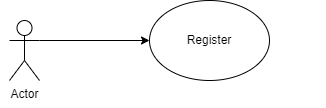
\includegraphics[height=5cm, width=0.8\textwidth]{./diagrams/Use Case/u1.png}
    \centering 
    \caption{Use Case Diagram for Registeration}
    \label{figure1}
    \end{figure}
    
    \begin{center}
        \begin{tabularx}{\textwidth}{|l|X|}
            \hline
            \textbf{ID} & UC-02 \\
            \hline
            \textbf{Name} & Register \\
            \hline
            \textbf{Description} & User can register their to keep their role in that software \\
            \hline
            \textbf{Actors} & New User \\
            \hline
            \textbf{Assumptions} & If user can Register, he/she will see more features \\
            \hline
            \textbf{Triggers} & Just Connect to in the internet and a email address \\
            \hline
            \textbf{Pre Conditions} & None \\
            \hline
            \textbf{Post Conditions} & Account Created Succesfully \\
            \hline
            \textbf{Main Course} & 1. Enter their Details 2.Create their accound according to their given details \\
            \hline
            \textbf{Alternative Course} & Error due to invalid details \\
            \hline
            
        \end{tabularx}
    \end{center}
    \newpage
    

    \subsubsection{UC-02: Login}
    \begin{figure}[H]
        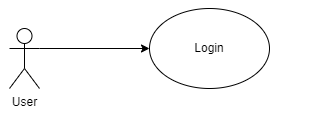
\includegraphics[height=5cm, width=0.8\textwidth]{./diagrams/Use Case/u2.png}
        \centering 
        \caption{Use Case Diagram for Login}
        \label{Usecase1}
        \end{figure}
        
    
    \begin{center}
        \begin{tabularx}{\textwidth}{|l|X|}
            \hline
            \textbf{ID} & UC-02 \\
            \hline
            \textbf{Name} & Login \\
            \hline
            \textbf{Description} & Login to the system to view/change in their account \\
            \hline
            \textbf{Actors} & New User \\
            \hline
            \textbf{Assumptions} & If user can login, he/she will use more features \\
            \hline
            \textbf{Triggers} & just confirm with email which they provided in sign up \\
            \hline
            \textbf{Pre Conditions} & they must have a account \\
            \hline
            \textbf{Post Conditions} & they succesfully see the dashboard and more settings and features \\
            \hline
            \textbf{Main Course} & User can enter/use their email and its valid password Check entered data and able to use \\
            \hline
            \textbf{Alternative Course} & Error due to invalid details \\
            \hline
            
        \end{tabularx}
    \end{center}
    \newpage
    

    \subsubsection{UC-03: OAuth}
    \begin{figure}[H]
        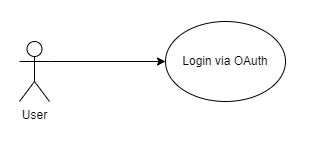
\includegraphics[height=5cm, width=0.8\textwidth]{./diagrams/Use Case/u3.png}
        \centering 
        \caption{Use Case Diagram for Login via OAuth}
        \label{Usecase1}
        \end{figure}
        
    \begin{center}
        \begin{tabularx}{\textwidth}{|l|X|}
            \hline
            \textbf{ID} & UC-03 \\
            \hline
            \textbf{Name} & OAuth \\
            \hline
            \textbf{Description} & User can ouath their details with third party like Gmail , LinkdIn and Github \\
            \hline
            \textbf{Actors} & New User \\
            \hline
            \textbf{Assumptions} & User can connect their third party account to login with the software \\
            \hline
            \textbf{Triggers} & just have a third party account  \\
            \hline
            \textbf{Pre Conditions} & none \\
            \hline
            \textbf{Post Conditions} & account has created by confiramtion through email  \\
            \hline
            \textbf{Main Course} & User can create their account on system by sending a email confirmation token. \\
            \hline
            \textbf{Alternative Course} & Error will show if you cant verify your Thir party account \\
            \hline
            
        \end{tabularx}
    \end{center}
    \newpage
    

    \subsubsection{UC-04: Forget Password}
    \begin{figure}[H]
        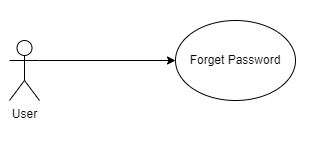
\includegraphics[height=5cm, width=0.8\textwidth]{./diagrams/Use Case/u4.png}
        \centering 
        \caption{Use Case Diagram for Forget Password}
        \label{fig: Usecase1}
        \end{figure}
        
    \begin{center}
        \begin{tabularx}{\textwidth}{|l|X|}
            \hline
            \textbf{ID} & UC-05 \\
            \hline
            \textbf{Name} & Forget Password \\
            \hline
            \textbf{Description} & Send the email to the user with a link to reset their password \\
            \hline
            \textbf{Actors} & Account Holder \\
            \hline
            \textbf{Assumptions} & An email is sent tu the user with a link to reset their password \\
            \hline
            \textbf{Triggers} &  \\
            \hline
            \textbf{Pre Conditions} & Valid Email \\
            \hline
            \textbf{Post Conditions} & New password has been changed \\
            \hline
            \textbf{Main Course} & User can change their password by sending link to their email and setting the new password with the password requirements \\
            \hline
            \textbf{Alternative Course} & Error will be show due to invalid details \\
            \hline
            
        \end{tabularx}
    \end{center}
    \newpage
    

    \subsubsection{UC-05: Reset Password}
    \begin{figure}[H]
        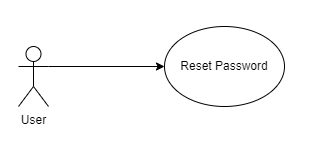
\includegraphics[height=5cm, width=0.8\textwidth]{./diagrams/Use Case/u5.png}
        \centering 
        \caption{Use Case Diagram for Reset Password}
        \label{fig:Usecase1}
        \end{figure}
        
    \begin{center}
        \begin{tabularx}{\textwidth}{|l|X|}
            \hline
            \textbf{ID} & UC-06 \\
            \hline
            \textbf{Name} & Reset Password \\
            \hline
            \textbf{Description} & User can reset your Password by entering you current password \\
            \hline
            \textbf{Actors} & Account Holder \\
            \hline
            \textbf{Assumptions} & To reset their password, User can enter the curent password and after confirmation it will be default password  \\
            \hline
            \textbf{Triggers} & Account Holder \\
            \hline
            \textbf{Pre Conditions} & user have a account \\
            \hline
            \textbf{Post Conditions} & password has been reset \\
            \hline
            \textbf{Main Course} & User can reset their password by entering their current password and password will set to default Password \\
            \hline
            \textbf{Alternative Course} & Error will be show due to invalid details \\
            \hline
            
        \end{tabularx}
    \end{center}
    \newpage
    

    \subsubsection{UC-06: Confirm Account}
    \begin{figure}[H]
        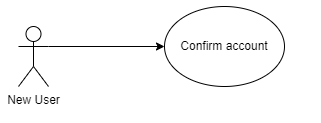
\includegraphics[height=5cm, width=0.8\textwidth]{./diagrams/Use Case/u6.png}
        \centering 
        \caption{Use Case Diagram for Confirm Account}
        \label{fig:Usecase1}
        \end{figure}
        
    \begin{center}
        \begin{tabularx}{\textwidth}{|l|X|}
            \hline
            \textbf{ID} & UC-07 \\
            \hline
            \textbf{Name} & Confirm Account \\
            \hline
            \textbf{Description} & User can confirm their account by a valid email address \\
            \hline
            \textbf{Actors} & New User \\
            \hline
            \textbf{Assumptions} &  \\
            \hline
            \textbf{Triggers} & By send the valid link to user's provided email \\
            \hline
            \textbf{Pre Conditions} & Fill the signup form \\
            \hline
            \textbf{Post Conditions} & account verified \\
            \hline
            \textbf{Main Course} & Account has been created though 3rd Party validation \\
            \hline
            \textbf{Alternative Course} & Error by unvalid email provided \\
            \hline
            
        \end{tabularx}
    \end{center}
    \newpage
    

    \subsubsection{UC-07: Delete Account}
    \begin{figure}[H]
        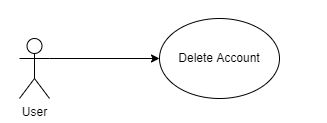
\includegraphics[height=5cm, width=0.8\textwidth]{./diagrams/Use Case/u7.png}
        \centering 
        \caption{Use Case Diagram for Delete Account}
        \label{fig:Usecase1}
        \end{figure}
        
    \begin{center}
        \begin{tabularx}{\textwidth}{|l|X|}
            \hline
            \textbf{ID} & UC-08 \\
            \hline
            \textbf{Name} & Delete Account \\
            \hline
            \textbf{Description} & User can delete the account if he/she can \\
            \hline
            \textbf{Actors} & Already User \\
            \hline
            \textbf{Assumptions} &  \\
            \hline
            \textbf{Triggers} & remove the user\_id from database by click on reset button \\
            \hline
            \textbf{Pre Conditions} & Already user database was be present in database \\
            \hline
            \textbf{Post Conditions} & No user of that user\_id will not be in database \\
            \hline
            \textbf{Main Course} & Account has been removed from database by the confirmation of user \\
            \hline
            \textbf{Alternative Course} & Error will be appeared by database \\
            \hline
            
        \end{tabularx}
    \end{center}
    \newpage
    

    \subsubsection{UC-08: Edit Account Info}
    \begin{figure}[H]
        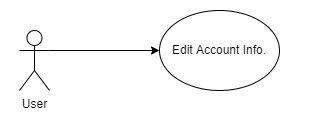
\includegraphics[height=5cm, width=0.8\textwidth]{./diagrams/Use Case/u8.png}
        \centering 
        \caption{Use Case Diagram for Edit Account Info}
        \label{fig:Usecase1}
        \end{figure}
        
    \begin{center}
        \begin{tabularx}{\textwidth}{|l|X|}
            \hline
            \textbf{ID} & UC-09 \\
            \hline
            \textbf{Name} & Edit Account Info \\
            \hline
            \textbf{Description} & User can edit their account information \\
            \hline
            \textbf{Actors} & Already User \\
            \hline
            \textbf{Assumptions} &  \\
            \hline
            \textbf{Triggers} & Database of that user can be updated \\
            \hline
            \textbf{Pre Conditions} & Already data of that user will be in database  \\
            \hline
            \textbf{Post Conditions} & Update the new version of their information in database \\
            \hline
            \textbf{Main Course} & Information of the User can be updated if he/she can \\
            \hline
            \textbf{Alternative Course} & Error willbe displaced by the Database \\
            \hline
            
        \end{tabularx}
    \end{center}
    \newpage 
    

    \subsubsection{UC-9: Edit Interface Preferences}
    \begin{figure}[H]
        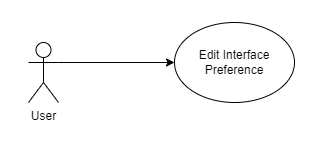
\includegraphics[height=5cm, width=0.8\textwidth]{./diagrams/Use Case/u9.png}
        \centering 
        \caption{Use Case Diagram for Edit Interface Preferences}
        \label{fig:Usecase1}
        \end{figure}
        
    \begin{center}
        \begin{tabularx}{\textwidth}{|l|X|}
            \hline
            \textbf{ID} & UC-10 \\
            \hline
            \textbf{Name} & Edit Interface Preferences \\
            \hline
            \textbf{Description} & User can edit their preferences of the UI of their dashboard \\
            \hline
            \textbf{Actors} & User \\
            \hline
            \textbf{Assumptions} &  \\
            \hline
            \textbf{Triggers} & User can change the primary and secondary Colors of the themes \\
            \hline
            \textbf{Pre Conditions} & Valid User \\
            \hline
            \textbf{Post Conditions} & UI preferences will be change according to User \\
            \hline
            \textbf{Main Course} & Interface preference will be changed by the user according to their preception  \\
            \hline
            \textbf{Alternative Course} & Error will be displayed it choose certain colors like black etc. \\
            \hline
            
        \end{tabularx}
    \end{center}
    \newpage
    

    \subsubsection{UC-10: Create Project}
    \begin{figure}[H]
        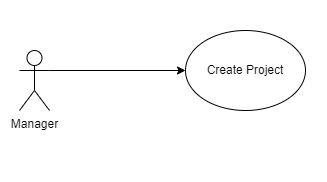
\includegraphics[height=5cm, width=0.8\textwidth]{./diagrams/Use Case/u10.png}
        \centering 
        \caption{Use Case Diagram for Create Project}
        \label{fig:Usecase1}
        \end{figure}
        
    \begin{center}
        \begin{tabularx}{\textwidth}{|l|X|}
            \hline
            \textbf{ID} & UC-11 \\
            \hline
            \textbf{Name} & Create Project \\
            \hline
            \textbf{Description} & Manager can create a project which is stored in the database with the unique id \\
            \hline
            \textbf{Actors} & Manager \\
            \hline
            \textbf{Assumptions} &  \\
            \hline
            \textbf{Triggers} & The Project will created in the database with unique id \\
            \hline
            \textbf{Pre Conditions} & user will be valid and Project can't created before  \\
            \hline
            \textbf{Post Conditions} & Project is created by the Manager \\
            \hline
            \textbf{Main Course} & Project is created by the manager in database \\
            \hline
            \textbf{Alternative Course} & Error will be displayed of database  \\
            \hline
            
        \end{tabularx}
    \end{center}
    
    \newpage

    \subsubsection{UC-11: Edit Project}
    \begin{figure}[H]
        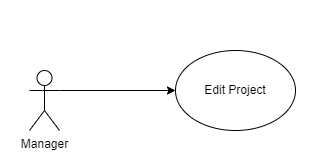
\includegraphics[height=5cm, width=0.8\textwidth]{./diagrams/Use Case/u11.png}
        \centering 
        \caption{Use Case Diagram for Edit Project}
        \label{fig:Usecase1}
        \end{figure}
        
    \begin{center}
        \begin{tabularx}{\textwidth}{|l|X|}
            \hline
            \textbf{ID} & UC-12 \\
            \hline
            \textbf{Name} & Edit Project \\
            \hline
            \textbf{Description} & The existing project will be edited by the manager if needed  \\
            \hline
            \textbf{Actors} & Manager \\
            \hline
            \textbf{Assumptions} &  \\
            \hline
            \textbf{Triggers} & The Information of the existing project will be updated in the database \\
            \hline
            \textbf{Pre Conditions} & Project is present already in database \\
            \hline
            \textbf{Post Conditions} & Project's Information will be updated by manager \\
            \hline
            \textbf{Main Course} & Manager can change the existing project if the requirements will be changed by the client \\
            \hline
            \textbf{Alternative Course} & Database's error will occurs \\
            \hline
            
        \end{tabularx}
    \end{center}
    \newpage
    

    \subsubsection{UC-12: Delete Project}
    \begin{figure}[H]
        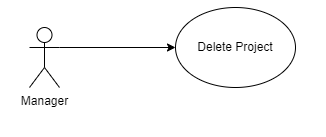
\includegraphics[height=5cm, width=0.8\textwidth]{./diagrams/Use Case/u12.png}
        \centering 
        \caption{Use Case Diagram for Delete Project}
        \label{fig:Usecase1}
        \end{figure}
        
    \begin{center}
        \begin{tabularx}{\textwidth}{|l|X|}
            \hline
            \textbf{ID} & UC-13 \\
            \hline
            \textbf{Name} & Delete Project \\
            \hline
            \textbf{Description} & The Manager will delete the existing projects from the database \\
            \hline
            \textbf{Actors} & Managers \\
            \hline
            \textbf{Assumptions} &  \\
            \hline
            \textbf{Triggers} & Delete the existing project from the database by delete event \\
            \hline
            \textbf{Pre Conditions} & Project will be in the database which Manager will be deleted \\
            \hline
            \textbf{Post Conditions} & Project is deletedby the the manager \\
            \hline
            \textbf{Main Course} & The manager will delete the exiting project which is presnet in database \\
            \hline
            \textbf{Alternative Course} & Error will be displayed \\
            \hline
            
        \end{tabularx}
    \end{center}
    \newpage
    

    \subsubsection{UC-13: Add Developer}
    \begin{figure}[H]
        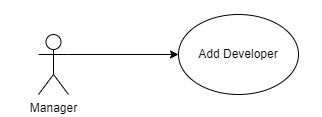
\includegraphics[height=5cm, width=0.8\textwidth]{./diagrams/Use Case/u13.png}
        \centering 
        \caption{Use Case Diagram for Add Developer}
        \label{fig:Usecase1}
        \end{figure}
        
    \begin{center}
        \begin{tabularx}{\textwidth}{|l|X|}
            \hline
            \textbf{ID} & UC-14 \\
            \hline
            \textbf{Name} & Add Developer \\
            \hline
            \textbf{Description} & The Manager will assign the developer of the company which is part of that Project \\
            \hline
            \textbf{Actors} & Managers \\
            \hline
            \textbf{Assumptions} &  \\
            \hline
            \textbf{Triggers} & Developer list will be shown to manager and manager will add the relevant developer \\
            \hline
            \textbf{Pre Conditions} & Developer and project will be added \\
            \hline
            \textbf{Post Conditions} & Developer will be added in the specific project \\
            \hline
            \textbf{Main Course} & To view the new upcoming project and take the decision of developer in project, Manager will added the developer in the project \\
            \hline
            \textbf{Alternative Course} & Error will be displayed \\
            \hline
            
        \end{tabularx}
    \end{center}
    
    \newpage

    \subsubsection{UC-14: Remove Developer}
    \begin{figure}[H]
        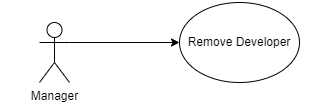
\includegraphics[height=5cm, width=0.8\textwidth]{./diagrams/Use Case/u14.png}
        \centering 
        \caption{Use Case Diagram for Remove Developer}
        \label{fig:Usecase1}
        \end{figure}
        
    \begin{center}
        \begin{tabularx}{\textwidth}{|l|X|}
            \hline
            \textbf{ID} & UC-15 \\
            \hline
            \textbf{Name} & Remove Developer \\
            \hline
            \textbf{Description} & The manager can remove the developer after developer performs their duties \\
            \hline
            \textbf{Actors} & Manager \\
            \hline
            \textbf{Assumptions} &  \\
            \hline
            \textbf{Triggers} & Manager will remove the developer in the project anytime. \\
            \hline
            \textbf{Pre Conditions} & Developer will be added in that project \\
            \hline
            \textbf{Post Conditions} & developer is no more the part of the project \\
            \hline
            \textbf{Main Course} & Manager can manage the availabilty of the developer whenever he enter in the project or when he exits. \\
            \hline
            \textbf{Alternative Course} & Error will be displayed \\
            \hline
            
        \end{tabularx}
    \end{center}
    \newpage
    

    \subsubsection{UC-15: Edit Developer Permission}
    \begin{figure}[H]
        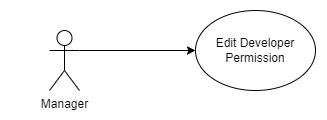
\includegraphics[height=5cm, width=0.8\textwidth]{./diagrams/Use Case/u15.png}
        \centering 
        \caption{Use Case Diagram for Edit Developer Permission}
        \label{fig:Usecase1}
        \end{figure}
        
    \begin{center}
        \begin{tabularx}{\textwidth}{|l|X|}
            \hline
            \textbf{ID} & UC-16 \\
            \hline
            \textbf{Name} & Edit Developer Permission \\
            \hline
            \textbf{Description} & The Manager can edit the role of the developer in the project \\
            \hline
            \textbf{Actors} & Managers \\
            \hline
            \textbf{Assumptions} &  \\
            \hline
            \textbf{Triggers} & Manager can edit the preference of the developer \\
            \hline
            \textbf{Pre Conditions} & Developer must have the part of the project \\
            \hline
            \textbf{Post Conditions} & Developer's Role will changed by the manager \\
            \hline
            \textbf{Main Course} & The Developer can change the role of the developer as he needs him in the project \\
            \hline
            \textbf{Alternative Course} & Error will be dislpayed by the database \\
            \hline
            
        \end{tabularx}
    \end{center}
    \newpage
    

    \subsubsection{UC-16: Calculate UCP}
    \begin{figure}[H]
        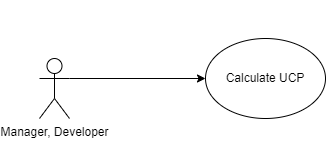
\includegraphics[height=5cm, width=0.8\textwidth]{./diagrams/Use Case/u16.png}
        \centering 
        \caption{Use Case Diagram for Calculate UCP}
        \label{fig:Usecase1}
        \end{figure}
        
    \begin{center}
        \begin{tabularx}{\textwidth}{|l|X|}
            \hline
            \textbf{ID} & UC-17 \\
            \hline
            \textbf{Name} & Calculate UCP \\
            \hline
            \textbf{Description} & Calculate the effort estimation of project via mean of UCP method \\
            \hline
            \textbf{Actors} & Manager , Developers \\
            \hline
            \textbf{Assumptions} &  \\
            \hline
            \textbf{Triggers} & The effort will calculted by UCP formula \\
            \hline
            \textbf{Pre Conditions} & The Project Use cases' information are inserted already \\
            \hline
            \textbf{Post Conditions} & Calculated Effort are given by UCP method  \\
            \hline
            \textbf{Main Course} & To find the Effort Estimation by UCP method of the entire project by the help of their use cases \\
            \hline
            \textbf{Alternative Course} & Error will displayed \\
            \hline
            
        \end{tabularx}
    \end{center}
    
    \newpage

    \subsubsection{UC-17: Get Machine Learning Estimation}
    \begin{figure}[H]
        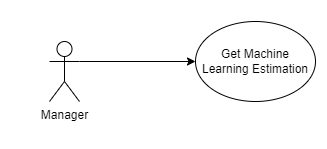
\includegraphics[height=5cm, width=0.8\textwidth]{./diagrams/Use Case/u17.png}
        \centering 
        \caption{Use Case Diagram for Get Machine Learning Estimation}
        \label{fig:Usecase1}
        \end{figure}
        
    \begin{center}
        \begin{tabularx}{\textwidth}{|l|X|}
            \hline
            \textbf{ID} & UC-18 \\
            \hline
            \textbf{Name} & Get Machine Learning Estimation \\
            \hline
            \textbf{Description} & Calculate the effort estimation of project via trained Machine Learning module \\
            \hline
            \textbf{Actors} & Manager  \\
            \hline
            \textbf{Assumptions} &  \\
            \hline
            \textbf{Triggers} & The effort will calculted by UCP formula \\
            \hline
            \textbf{Pre Conditions} & The Project Use cases' information are inserted already \\
            \hline
            \textbf{Post Conditions} & Calculated Effort are given by UCP method  \\
            \hline
            \textbf{Main Course} & To find the Effort Estimation by UCP method of the entire project by the help of their use cases \\
            \hline
            \textbf{Alternative Course} & Error will displayed \\
            \hline
            
        \end{tabularx}
    \end{center}
    \newpage
    

    \subsubsection{UC-18: Manual Estimate Round}
    \begin{figure}[H]
        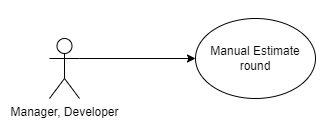
\includegraphics[height=5cm, width=0.8\textwidth]{./diagrams/Use Case/u18.png}
        \centering 
        \caption{Use Case Diagram for Manual Estimate Round}
        \label{fig:Usecase1}
        \end{figure}
        
    \begin{center}
        \begin{tabularx}{\textwidth}{|l|X|}
            \hline
            \textbf{ID} & UC-19 \\
            \hline
            \textbf{Name} & Manual Estimate Round \\
            \hline
            \textbf{Description} & Calculate the effort estimation of project via Manual Estimation where the developer and experts will estimate the project while round \\
            \hline
            \textbf{Actors} & developers, manager \\
            \hline
            \textbf{Assumptions} &  \\
            \hline
            \textbf{Triggers} & The Effort will calculated by Manual technique \\
            \hline
            \textbf{Pre Conditions} & Developers were added by manager  in the project \\
            \hline
            \textbf{Post Conditions} & The effort will calculated after the many rounds of the experts' discussions  \\
            \hline
            \textbf{Main Course} & To find the Effort estimation by Manual technique by many rounds \\
            \hline
            \textbf{Alternative Course} & Error will displayed \\
            \hline
            
        \end{tabularx}
    \end{center}
    
    \newpage

    \subsubsection{UC-19: Estimation Bar}
    \begin{figure}[H]
        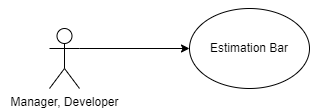
\includegraphics[height=5cm, width=0.8\textwidth]{./diagrams/Use Case/u19.png}
        \centering 
        \caption{Use Case Diagram for Estimation Bar}
        \label{fig:Usecase1}
        \end{figure}
        
    \begin{center}
        \begin{tabularx}{\textwidth}{|l|X|}
            \hline
            \textbf{ID} & UC-20 \\
            \hline
            \textbf{Name} & Estimation Bar \\
            \hline
            \textbf{Description} & All Estimation will be shown in the form of graphs \\
            \hline
            \textbf{Actors} & Manager , Developer \\
            \hline
            \textbf{Assumptions} &  \\
            \hline
            \textbf{Triggers} & The Estimate will be generated by the experts' round discussion \\
            \hline
            \textbf{Pre Conditions} & The estimation will be measured before that step  \\
            \hline
            \textbf{Post Conditions} & The charts will be appeared \\
            \hline
            \textbf{Main Course} & Estimation will be deliver in bar that anyone will be see and clearly judge the estimation of the project \\
            \hline
            \textbf{Alternative Course} & Error wil be displayed \\
            \hline
            
        \end{tabularx}
    \end{center}
    \newpage
    

  